\subsection{HTML} % (fold)
\label{sub:html}

Since the very beginning, \ida{HTML} has been the soul of the \ida{WWW}.
Created by \emph{Tim Berners-Lee} at \emph{CERN} around 1990, this markup language was aimed at providing an hypertext digital solution.
The beauty of an hypertext document is that it can contain references (hyperlinks) to other documents, so a person or computer can navigate easily though the documents in a non-linear way, normally from a remote computer.

The most popular way to view these documents is using a Web Browser.
There are several vendors that offer competing products, but the main ones have been evolved following closely the growth of the web.
These browsers interpret the code and generate a visual (or audible) representation suitable for human consumption.

Typically \ida{HTML} pages are delivered using \ida{HTTP}, the protocol specifically designed for this purpose.
Additional resources are also delivered this way, e.g., images, scripts or stylesheets.
Every document has a unique address (\ida{URL}) that allows the browser to find in which remote machine is located (usually a server), which path has to ask for and which further parameters are needed.

The language itself is based on \ida{SGML}, father of the more popular (and realistic) \ida{XML}.
Documents written in these languages are composed by elements consisting of \emph{tags} within the page content in a plain text file.

The name of these tags are enclosed in angle brackets (like \texttt{<div>}), and normally they come in pairs: one at the beginning (the opening tag) and one at the end (the closing tag, like the opening tag but with a backslash, e.g. \texttt{</div>}).

Each tag can contain different attributes that will affect that particular tag.
The actual content goes between those two tags, and that content can be a combination of plain text and other tags (children of that element).
Therefore a document can be represented as a tree, with each element acting as a node and having \texttt{<html>} as the parent node.

The following line shows an example element.
It has two different attributes, one called \idc{id} and other called \idc{class}, and each one has a different value.
The meaning and usefulness of these attributes will be discussed later.

\texttt{<div id="myid" class="myclass"}\texttt{>Text</div>}

A document consists of two sections: the head and the body.
The head contains the metadata of the document (title, language, encoding, styles, scripts, etc) and its content is not displayed in the browser.
By contrast the body is where the content goes.

Over the years a diverse range of \ida{HTML} tags have been supported, either promoted by a standards body or unilaterally by browser vendors.
Now there are tags for embedding multimedia content (images, video, audio), tables, forms, headings, paragraphs, comments, lists, quotes, code, etc.
Of course, also links and even other full pages using frames.

Besides these content related tags, there are also tags to specify the appearance and layout of the page (\ida{CSS}) and its behavior (\idx{JavaScript}).
Since this code does not relate to the content itself, it is best to put it in external files and just link them from the \ida{HTML}.
Table~\vref{tab:htmlelements} shows a comprehensive list of the most used elements in current web pages.
On the other hand, Listing~\vref{phpexampleafter} shows how an \ida{HTML} document looks like.

\begin{invisibletable}[\idx{HTML} elements]{4}
  {p{0.15\textwidth} p{0.15\textwidth} p{0.15\textwidth} p{0.15\textwidth}}
  \label{tab:htmlelements}%
  \texttt{html} & \texttt{head} & \texttt{body} & \texttt{title} \\
  \texttt{meta} & \texttt{object} & \texttt{script} & \texttt{p} \\
  \texttt{h1...h6} & \texttt{ul} & \texttt{ol} & \texttt{li} \\
  \texttt{blockquote} & \texttt{pre} & \texttt{div} & \texttt{span} \\
  \texttt{a} & \texttt{em} & \texttt{strong} & \texttt{code} \\
  \texttt{br} & \texttt{hr} & \texttt{img} & \texttt{form} \\
  \texttt{input} & \texttt{select} & \texttt{textarea} & \texttt{iframe} \\
  \texttt{table} & \texttt{tr} & \texttt{th} & \texttt{td} \\
\end{invisibletable}

Each of these elements may specify a different set of attributes, name-value pairs separated by a `=' symbol written within the start tag of the element after the element's name.
The most important attributes are \idc{id} and \idc{class}, and they can apply to every element.
Most other attributes are useful only for one or two elements.

The former specifies a unique identifier for that element, so it could be easily modified by \ida{CSS} rules and \idx{JavaScript} code.
Additionally, it allows to link directly to that element rather than to the full page putting its identifier at the end of address after the `\#' character.

The latter indicates that the element belongs to one or more classes.
Classes are used to classify and group similar elements for semantic or presentation purposes, something very useful for \ida{CSS} but also for \idx{JavaScript}.
Multiple class values can be assigned by separating their names with spaces (\texttt{"class1 class2 class3"}).

This standard has been traditionally maintained in the \ida{W3C}, the primary international organization for the \ida{WWW}.
The most popular version is \ida{HTML} 4 (and its subsequent minor revision \ida{HTML} 4.01), the only version that it is also an \ida{ISO} standard  \cite{HTML4}.
A parallel version with the same capabilities but based on well formatted \ida{XML} was released as \ida{XHTML} 1.0 and later \ida{XHTML} 1.1  \cite{HTML4}.

After several years of stalled development making the \ida{XHTML} 2.0 specification, some browser vendors got tired of waiting and founded the \ida{WHATWG}.
Through this new standardization body \ida{HTML} 5 was born, and later the \ida{W3C} dropped \ida{XHTML} 2.0 and declared \ida{HTML} 5 to be the official evolution of \ida{HTML}.
More information about this new standard is stated in \S\vref{sub:html5css3}.

Every version is mostly compatible with the previous one, but some subtle differences make browsers need a way to distinguish between them.
For that a well formed \ida{HTML} document must start with the \idc{doctype}.
This is a tag that needs to be put at the very beginning of the document, defining which standard the document follows.
Listing~\vref{phpexampleafter} showed the standard \ida{HTML} 5 \idc{doctype}.

When the page is parsed by a browser, it starts believing that the document complies with this \idc{doctype}, and the rendering is relatively predictable according to the specification.
However, given the large quantity of malformed pages\footnote{This vicious cycle is also the browsers' fault, because their parsers have been historically very lenient about \ida{HTML} errors in order to be compatible with more pages.}, in many occasions it sadly backfires to a quirks mode.
As opposed to the standard mode, this mode is mostly unpredictable, and it usually leads to strange bugs and inconsistent states.

This situation gets worse because traditionally different browsers provide contradictory support (or no support at all) of some parts of the specification, especially \ida{CSS}.
\ida{IE} is the worst offender in this aspect, not only for the engine itself, but because it took more than five years until \idx{Microsoft} finally released a new version.
During that time, every non security bug remained unfixed in the default browser that shipped with almost every computer.

Due to the huge market share held by \ida{IE} (see Figure~\vref{fig:browser-ie-share})\footnote{Data extracted from \emph{Statcounter GlobalStats}: \url{http://gs.statcounter.com/}. It may be a little biased towards modern browsers but trends match other sources.}, this has been the primary frustration for every front end developer, and a tremendous drawback for web applications.
For instance, in this work a considerable amount of development time was spent bypassing \ida{IE} bugs, and from the beginning it was decided to drop \ida{IE}6 support, a browser in clear decline not even fully supported by \idx{Microsoft}.

New \ida{IE} versions are slowly reverting that situation with a more modern and standards based engine, and for developers rejoice the market share of \ida{IE}6 is rapidly declining (see Figure~\vref{fig:browser-ie-share}).
However, it is probable that as long as \ida{IE}6/7/8 and \idx{Windows XP} retain any substantial market share, web developers will continue supporting effectively 3 or 4 ostensibly different engines only from \idx{Microsoft}, plus the competition.

\begin{figure}[htbp]
  \centering
  \subfigure[Market share of the top five browsers]{
    \label{fig:browser-share}
    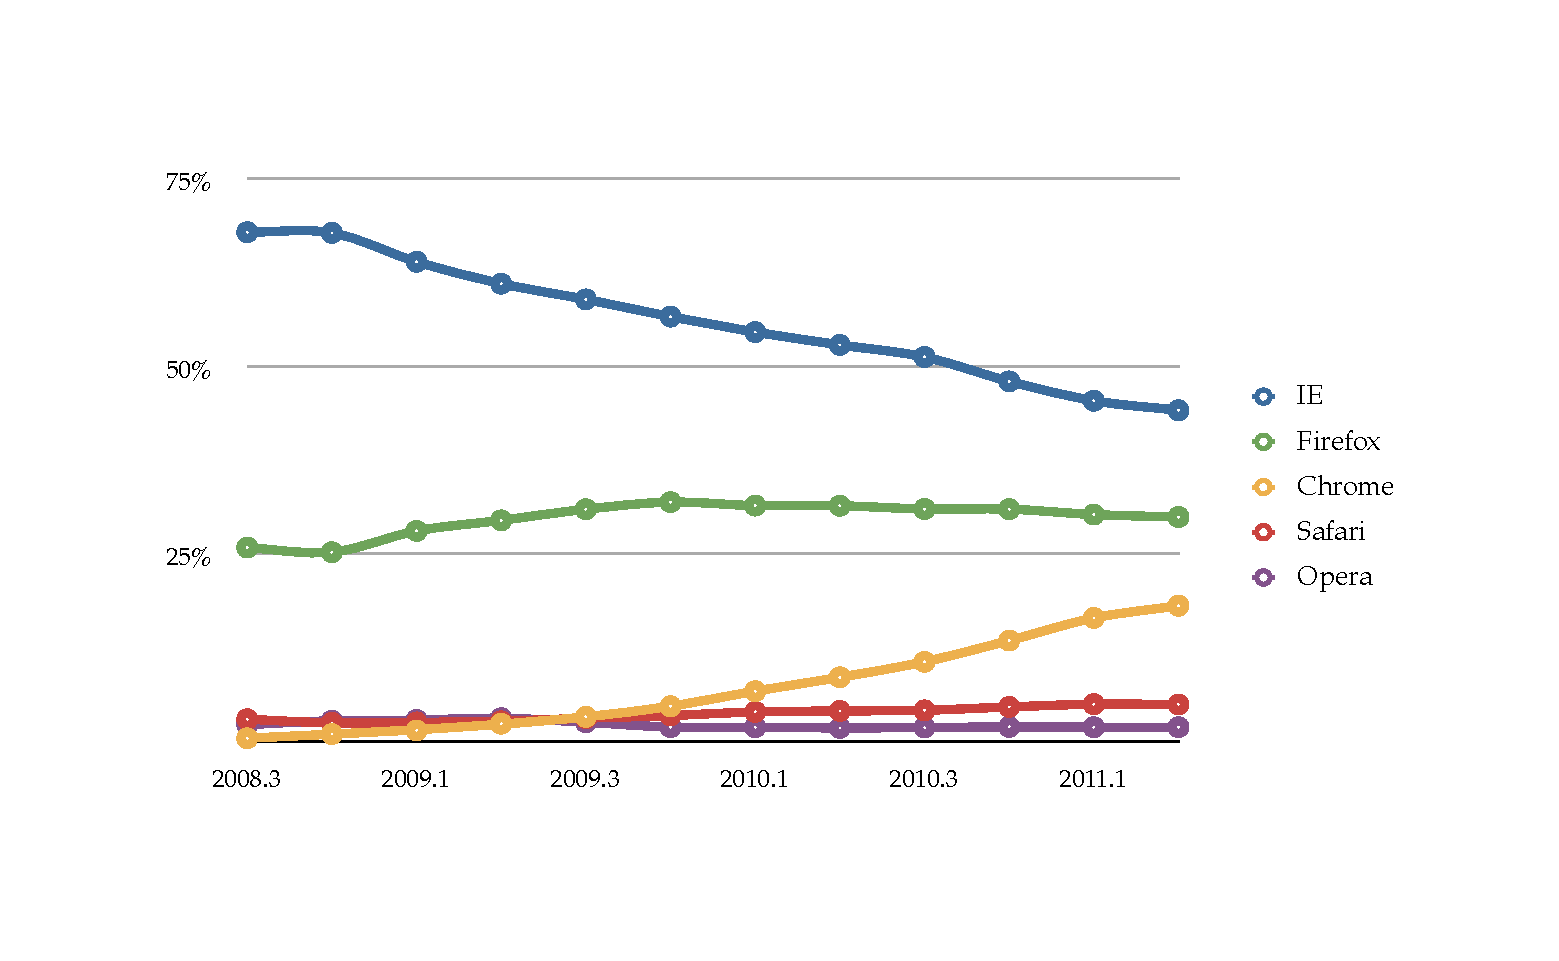
\includegraphics[width=\textwidth]{browser-share}
  }
  \subfigure[Market share of current versions of IE]{
    \label{fig:browser-ie-share}
    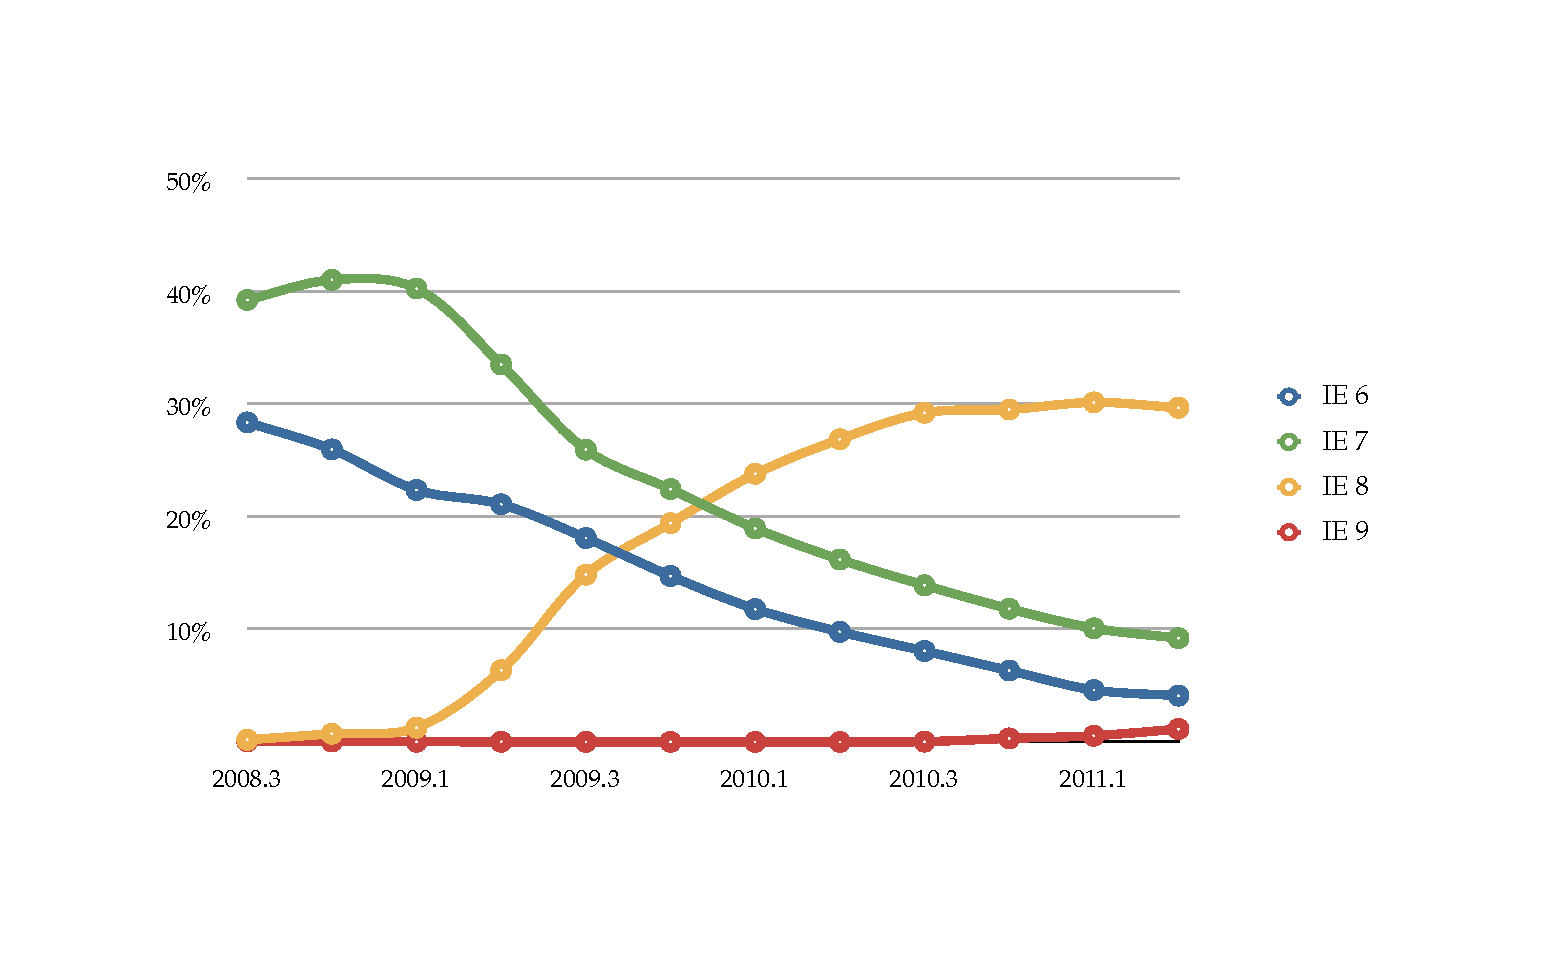
\includegraphics[width=\textwidth]{browser-ie-share}
  }
  \caption{Current browser market shares and trends}
  \label{fig:browser-trends}
\end{figure}

% subsection html (end)